\chapter{Curvature and Differential Geometry}
\label{chap:curvature}

\begin{Abstract}
A discussion of both line and surface curvature is a core feature in the subject of 
differential geometry. See, for example, books \cite{Oprea_2007_DGA}, \cite{Davies_1996_CGCS}, and \cite{doCarmo_1976_DGCS}. Studies on 
surface curvature can be traced back to original work by Gauss; see, for example, 
\cite{Pesic_2005_GICS}. This chapter begins with a review of curvature basics, establishes 
notational conventions, and adds a few new results (e.g., on n-cuts). The chapter continues with a new scale invariant curvature 
measure and concludes with a presentation of some curvature visualization examples.
\end{Abstract}

%---------------- section ----------------
\section{Notational Conventions}
In writing this book, a challenge encountered, because of synthesizing multiple disciplines, was differences in standard notation, sometimes subtle, but none the less significant. We chose to employ vector notation and homogeneous coordinates\footnote{The use of homogeneous coordinates facilitates the general use of transformation matrices.} for both points and directions. Point and directions are thus instances of an abstract vector class in which the fourth coordinate for points is one, and the forth coordinate for directions is zero.\\

%+++++++++++++++++++++++++++++++++++++++++
\begin{figure}[!t]
\begin{center}
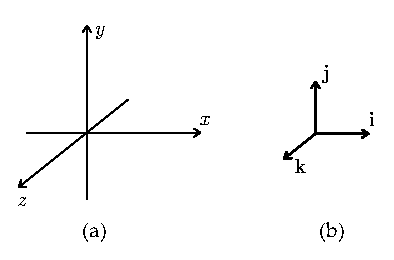
\epsfig{file=chapters/Introduction/axes, height=40mm}
\end{center}
\vspace{-12pt}
\caption{Right-handed $y$-up coordinate system and the associated unit basis vectors.}
\label{fig:introduction-axes}
\end{figure}
%+++++++++++++++++++++++++++++++++++++++++

We assign a \emph{right-handed $y$-up} orthogonal coordinate system to 3D space as shown in Figure \ref{fig:introduction-axes}. By convention, the \emph{$\mathbf{i}\mathbf{j}\mathbf{k}$ unit basis vectors} align with the positive direction of the $x y z$ axes respectively.\\

\section{Curves and Arcs}
\label{sec:curvature-curves}
We consider \emph{closed simple curves} in 3D space. Such curves can be specified parametrically as a set of points
\begin{equation}
A = \left\{ \mathbf{p}(t) =
\left[
\begin{array}{c}
x(t) \\
y(t) \\
z(t)
\end{array}
\right]
:
t_{min} \le t < t_{max}
\right\}
\end{equation}
where $\mathbf{p}(t)$ is a continuous function, $\mathbf{p}(t_1) \ne \mathbf{p}(t_2)$ for 
all $t_1 \ne t_2$, and \\$\lim_{(t \rightarrow t_{max})}\mathbf{p}(t) = 
\mathbf{p}(t_{min})$. A point\footnote{In this work, we use vector notation for both 
points and directions.} in the curve can be referred to as point $\mathbf{p}$.\\

Example (a) in Figure~\ref{fig:curvature-curves} is a closed, simple curve. Note that the points in (a) form a closed loop. Curve (b) does not meet the $\lim_{(t \rightarrow t_{max})}$ criterion and is thus not closed. Curve (c) is self intersecting (i.e., $\mathbf{p}(t_1)=\mathbf{p}(t_2)$ for some $t_1 \ne t_2$) and is thus not simple. \\

%+++++++++++++++++++++++++++++++++++++++++
\begin{figure}[!t]
\begin{center}
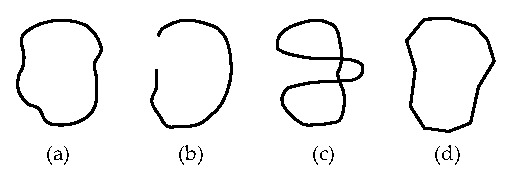
\epsfig{file=chapters/Curvature/curves, height=30mm}
\end{center}
\caption{(a) Closed, simple, smooth curve. (b) Not closed. (c) Not simple. (d) Not smooth.}
\label{fig:curvature-curves}
\end{figure}
%+++++++++++++++++++++++++++++++++++++++++

The points in a curve are \emph{ordered} in the sense that if $t_1<t_2<t_3$ then $\mathbf{p}(t_1)<\mathbf{p}(t_2)<\mathbf{p}(t_3)$. Thus we can construct sequences of points in a curve as well as consider limits such as $\lim_{\mathbf{p} \to \mathbf{p_0}}$.\\

A curve is called \emph{smooth} if the function $\mathbf{p}(t)$ is continuously differentiable. We define differentiability at the point $\mathbf{p}(t_{min})$ by considering a \emph{shifted} parameterization with $(t_{min}-\delta) \le t < (t_{max}-\delta)$ for some $\delta > 0$, thus extending the domain of the function $\mathbf{p}(t)$, such that $\mathbf{p}(t_{min}-\varepsilon) = \mathbf{p}(t_{max}-\varepsilon)$ whenever $0 < \varepsilon \le \delta$. Curve (d) in Figure~\ref{fig:curvature-curves} contains some corner points and is thus not smooth. \\

Using the notational convention $\dot{x} = dx / dt$, the \emph{speed} of a curve parameterization at the point $\mathbf{p}$ is given by the following:
\begin{equation}
s(t) = ||\mathbf{\dot{p}}|| = \sqrt{(\dot{x})^2 + (\dot{y})^2 + (\dot{z})^2}
\label{eq:curvature-speed}
\end{equation}

A curve parameterization $\mathbf{p}(t)$ is said to be \emph{regular} if its speed is never zero. Any point $\mathbf{p}(t)$ at which the speed of a curve parameterization is zero is said to be a \emph{singular point} under that parameterization. Some singularities are removable under a change of parameterization; others are not removable.\\

\emph{By default, in this work, when we refer to a curve, we mean a smooth closed simple curve that has a regular parameterization.}\\

We define an \emph{arc} as any subset of a curve where that subset is parameterized by $t$ with $a \le t \le b$ and $t_{min} \le a < b < t_{max}$. The \emph{end-points} of the arc are $\mathbf{p}(a)$ and $\mathbf{p}(b)$. Arcs that include the point $\mathbf{p}(t_{min})$ can be constructed using a shift in parameterization as given in the previous discussion of differentiabily.\\

In general, the \emph{arc-length} of an arc is given by the following:
\begin{equation}
\int_{a}^{b} s(t)\, dt
\end{equation}

Arc-length can alternatively be considered as a function of $t$ where the length is that from some starting point in a curve, parameterized by $t_{0}$, to an \emph{arbitrary point} in the curve parameterized by $t$:
\begin{equation}
\label{eq:curvature-arclength}
l(t) = \int_{t_{0}}^{t} s(t)\, dt
\end{equation}
Note that arc-length is independent of the particular curve parameterization that is used. We will additionally restrict our consideration of curves to only those not containing infinite length arcs. This eliminates so-called \emph{space filling curves}\footnote{An example is the \emph{Peano curve} which fills the entire unit square.}.\\

The following is a basic theorem from differential geometry.
\begin{theorem}
A regular curve reparameterized by arc-length has unit speed at all points.
\end{theorem}

This reparameterization can be written as
\begin{equation}
A = \left\{ \mathbf{p}\big(t(l)\big) =
\left[
\begin{array}{c}
x\big(t(l)\big) \\
y\big(t(l)\big) \\
z\big(t(l)\big)
\end{array}
\right]
:
0 \le l < l(t_{max})
\right\}
\end{equation}
Note that, to write this reparameterization explicitly, we need to solve Equation~(\ref{eq:curvature-arclength}) for $t$, and this is not always possible.

\begin{definition}
The (unit length) \emph{tangent direction vector} to a curve at point $\mathbf{p}$ is given by the following:
\begin{equation}
\mathbf{\hat{t}} = \frac{\mathbf{\dot{p}}}{|| \mathbf{\dot{p}} ||}
\end{equation}
\end{definition}

There is a unique \emph{tangent line} associated with each point $\mathbf{p}_0$ on a curve. The tangent line is the set of points given by
\begin{equation}
\label{eq:curvature-line}
L = \left\{ \mathbf{p}(t) =
\mathbf{p}_0 + \mathbf{\hat{t}} \, t
:
-\infty < t < +\infty
\right\}
\end{equation}
The tangent line to a curve at a given point is independent of the parameterization used.\\

Whenever a line is specified in the form of Equation~(\ref{eq:curvature-line}), both a reference point $\mathbf{p}_0$ and a direction vector $\mathbf{\hat{t}}$ are given. Note that, in general, for any specific line (set of points), the reference point $\mathbf{p}_0$ could be any point on the line (one of an infinite number of possibilities) and direction vector could be $\pm \mathbf{\hat{t}}$ (one of exactly two possibilities).\\

\begin{definition}
The (unit length) \emph{normal direction vector} to a curve at point $\mathbf{p}$ is given by the following:
\begin{equation}
\mathbf{\hat{n}} = \frac{\mathbf{\dot{\hat{t}}}}{|| \mathbf{\dot{\hat{t}}} ||}
\end{equation}
\end{definition}

Note that the normal vector is undefined both at points where the tangent function is not differentiable and (because of a divide by zero) within any arc where the tangent vector is constant. Also, a basic result from differential geometry shows that, at each point in a curve, the normal vector, where defined, \emph{is orthogonal to the associated tangent vector}.\\

%------------- subsection ----------------
\subsection{Curvature of Plane Curves}
\label{sec:curvature-plane-curves}

Even though, in this section, we focus on plane curves, we will work in $\mathbb{R}^3$ because we seek properties that are generally applicable in 3D space.\\

%+++++++++++++++++++++++++++++++++++++++++
\begin{figure}[!t]
\begin{center}
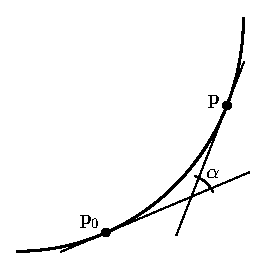
\epsfig{file=chapters/Curvature/curvature1, height=40mm}
\end{center}
\caption{Curvature at the point $\mathbf p_0$ is defined in the limit $\mathbf p \rightarrow \mathbf p_0$.}
\label{fig:curvature-curvature1}
\end{figure}
%+++++++++++++++++++++++++++++++++++++++++

\begin{definition}
Consider a plane curve with arc-length $l$ from the point $\mathbf p_0$ to the point $\mathbf p$, and the (non-negative) angle $\alpha$ between the tangent lines at $\mathbf p_0$ and $\mathbf p$ as illustrated, for example, in Figure~\ref{fig:curvature-curvature1}. Then the \emph{curvature} of the curve at point $\mathbf p_0$ is defined to be
\begin{equation}
\kappa = \lim_{\mathbf p \rightarrow \mathbf p_0} \frac{\alpha}{l} = \frac{d\alpha}{dl}
\end{equation}
\end{definition}
Note that curvature as defined here is always non-negative. Since neither the angle between the tangent lines, nor the arc-length, are altered by translation and rotation, we conclude that curvature is a translation and rotation independent property.\\

%+++++++++++++++++++++++++++++++++++++++++
\begin{figure}[!t]
\begin{center}
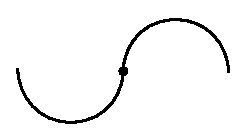
\epsfig{file=chapters/Curvature/k_undefined, height=25mm}
\end{center}
\caption{Curvature is not defined at the join point of two half circles.}
\label{fig:curvature-k_undefined}
\end{figure}
%+++++++++++++++++++++++++++++++++++++++++

Curvature is not necessarily defined at all points on a smooth curve. A well-known result gives constant curvature $1/r$ at all points of a circle having radius $r$. However, for example, curvature is not defined at the joining point of the arc constructed from two half circles, even when both have the same radius, as shown in Figure~\ref{fig:curvature-k_undefined}. The existence of curvature at a point is conditional on a parameterization having a continuous second derivative at that point.\\

We show, in the following example, that the second derivative for this curve is not continuous.\\

%+++++++++++++++++++++++++++++++++++++++++
\begin{figure}[!t]
\begin{center}
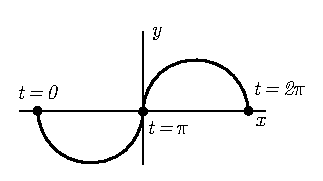
\epsfig{file=chapters/Curvature/param_k_undefined, height=25mm}
\end{center}
\caption{A parameterization for an arc constructed from two half circles.}
\label{fig:curvature-param_k_undefined}
\end{figure}
%+++++++++++++++++++++++++++++++++++++++++

Consider the arc, constructed from joining two unit radius half-circles as shown in Figure~\ref{fig:curvature-param_k_undefined}, parameterized by:

\begin{equation}
\mathbf{p}(t)=
\left\{
\begin{array}{ll}
0 \le t \le \pi & \quad
\left[\begin{array}{c}
\cos (t - \pi)\\
\sin (t - \pi)
\end{array}\right]
- \left[ \begin{array}{c} 1\\0 \end{array} \right]\\
\\
\pi < t \le 2\pi & \quad
\left[\begin{array}{c}
\cos (-t)\\
\sin (-t)
\end{array}\right]
+ \left[ \begin{array}{c} 1\\0 \end{array} \right]\\
\end{array}
\right.
\end{equation}\\

When $0 \le t \le \pi$ we have:
\begin{align}
\dot{\mathbf{p}}(t) &=
\left[\begin{array}{c}
- \sin (t - \pi)\\
\cos (t - \pi)
\end{array}\right]\\
\ddot{\mathbf{p}}(t) &=
\left[\begin{array}{c}
- \cos (t - \pi)\\
- \sin (t - \pi)
\end{array}\right]
\end{align}

Making use of the identities $\cos (-t) = \cos (t)$ and $\sin (-t) = -\sin (t)$, we have, when $\pi < t \le 2\pi$ :
\begin{align}
\dot{\mathbf{p}}(t) &=
\left[\begin{array}{c}
- \sin (t)\\
- \cos (t)
\end{array}\right]\\
\ddot{\mathbf{p}}(t) &=
\left[\begin{array}{c}
- \cos (t)\\
\sin (t)
\end{array}\right]
\end{align}

When $t = \pi$, both of the first derivatives evaluate to
$\footnotesize \Bigl[ \begin{array}{c} 0\\1 \end{array} \Bigr]$
. Thus, the first derivative of the arc, as a whole, is continuous at the join-point.
However, again when $t = \pi$, the second derivatives evaluate to
$\footnotesize \Bigl[ \begin{array}{c} -1\\0 \end{array} \Bigr]$
and
$\footnotesize \Bigl[ \begin{array}{c} 1\\0 \end{array} \Bigr]$ respectively. Since the second derivative of the arc parameterization is not continuous at the join point, curvature is not defined there.\\

Note that there is also a related discontinuity in the direction of the normal vector $\mathbf{\hat{n}}$ at the join point.\\

The following theorem from differential geometry summarizes a useful relationship involving curvature.
\begin{theorem}
The \emph{Frenet formula},
\begin{equation}
\label{eq:frenet1}
\left[
\begin{array}{c}
\mathbf{\dot{\hat{t}}} \\
\mathbf{\dot{\hat{n}}}
\end{array}
\right]
=
\left[
\begin{array}{cc}
0 & ks \\
-ks & 0
\end{array}
\right]
\left[
\begin{array}{c}
\mathbf{\hat{t}} \\
\mathbf{\hat{n}}
\end{array}
\right]
\end{equation}
describes the relationship between the curvature, speed, the  tangent and the normal at each point in a planar curve.
\end{theorem}

Since any plane curve in $\mathbb{R}^3$ can be transformed by rotation and translation such that it lies in the $xy$ coordinate plane, it is meaningful, for curvature calculation purposes, to consider $xy$ plane curves.\\

Curvature for an $xy$-plane curve can be computed directly, from the curve parameterization, as
\begin{equation}
k = \frac{|\dot{x}\ddot{y} - \ddot{x}\dot{y}|}{(\dot{x}^2+\dot{y}^2)^{3/2}}
\end{equation}
or for a unit speed parameterization as simply
\begin{equation}
k = |\dot{x}\ddot{y} - \ddot{x}\dot{y}|
\end{equation}

Curvature for $xy$-plane curves, given as a function $y(x)$ in rectangular coordinates, can be computed as
\begin{equation}
k = \frac{|\frac{d^2y}{dx^2}|}{(1+(\frac{dy}{dx})^2)^{3/2}}
\end{equation}
and for plane curves given as $r(\theta)$ in polar coordinates as
\begin{equation}
k = \frac{r^2 + 2 \, (\frac{dr}{d\theta})^2 - r^2 \, |\frac{d^2r}{d\theta^2}|}{(r^2+(\frac{dr}{d\theta})^2)^{3/2}}
\end{equation}

Note that curvature is dependent in general on both first and second order derivatives.\\

%------------- subsection ----------------
\subsection{Curvature and Planar Regions}
\label{sec:curvature-planar-regions}

%+++++++++++++++++++++++++++++++++++++++++
\begin{figure}[!t]
\begin{center}
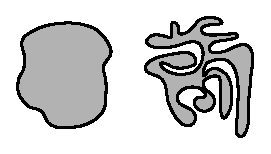
\epsfig{file=chapters/Curvature/regions, height=30mm}
\end{center}
\vspace{-10pt}
\caption{Closed simple curves and associated interior regions.}
\label{fig:curvature-regions}
\end{figure}
%+++++++++++++++++++++++++++++++++++++++++

A closed simple planar curve separates the plane into two regions: a bounded \emph{interior} and an unbounded \emph{exterior}. Figure~\ref{fig:curvature-regions} shows two curves, each with its associated interior region shaded.\\

In this work, we associate a (closed simple) planar curve, as well as each of its arcs, 
with its interior region.\\

A preliminary definition is required before we reconsider curvature.

\begin{definition}
The (planar) \emph{$\varepsilon$-neighborhood} of a point $\mathbf{p}$ in a plane is the open disk of all points in the plane whose distance to $\mathbf{p}$ is less than $\varepsilon$.
\end{definition}

%+++++++++++++++++++++++++++++++++++++++++
\begin{figure}[!t]
\begin{center}
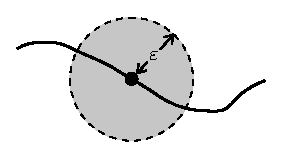
\epsfig{file=chapters/Curvature/neighborhood, height=20mm}
\end{center}
\vspace{-10pt}
\caption{A planar $\varepsilon$-neighborhood (open disk).}
\label{fig:curvature-neighborhood}
\end{figure}
%+++++++++++++++++++++++++++++++++++++++++

Figure~\ref{fig:curvature-neighborhood} illustrates the $\varepsilon$-neighborhood of a point in an arc.\\

The association of an interior region with a curve allows us to refine our definition of curvature, from Section~\ref{sec:curvature-plane-curves}, with an assignment of a \emph{polarity sign}.

\begin{definition}
Consider the non-zero curvature at a point \emph{$\mathbf{p}$} on a curve and the tangent line at that point. A \emph{negative polarity} is assigned to that curvature if there exists an $\varepsilon$-neighborhood of \emph{$\mathbf{p}$} such that, within that $\varepsilon$-neighborhood, all of the points of the tangent line, except for \emph{$\mathbf{p}$} itself, are part of the associated interior region. The curvature has a \emph{positive polarity} otherwise.
\end{definition}

%+++++++++++++++++++++++++++++++++++++++++
\begin{figure}[!t]
\begin{center}
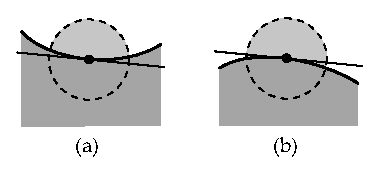
\epsfig{file=chapters/Curvature/polarity, height=30mm}
\end{center}
\vspace{-10pt}
\caption{(a) Negative curvature. (b) Positive curvature.}
\label{fig:curvature-polarity}
\end{figure}
%+++++++++++++++++++++++++++++++++++++++++

Figure~\ref{fig:curvature-polarity} illustrates the definition of curvature polarity. It shows example arcs, interior regions, $\varepsilon$-neighborhoods, and tangents lines for each of the two curvature polarity possibilities.\\

Throughout the remainder of this book, a polarity will always be assigned to (non-zero) curvature.\\

%---------------- section ----------------
\section{Surfaces and Surface Patches}
Consider \emph{closed simple surfaces} in 3D space. Such a surface can be specified parametrically as a set of points
\begin{equation}
S = \left\{ \mathbf{p}(u,v) =
\left[
\begin{array}{c}
x(u,v) \\
y(u,v) \\
z(u,v)
\end{array}
\right]
:
(u_{min} \le u < u_{max})  \, \wedge \,
(v_{min} \le v < v_{max})
\right\}
\end{equation}
where $\mathbf{p}(u,v)$ is a continuous function, $\mathbf{p}(u_1,v_1) \ne \mathbf{p}(u_2,v_2)$ for all $(u_1,v_1) \ne (u_2,v_2)$, $\forall(v) (\lim_{(u \rightarrow u_{max})}\mathbf{p}(u,v) = \mathbf{p}(u_{min},v))$, and $\forall(u) (\lim_{(v \rightarrow v_{max})}\mathbf{p}(u,v) = \mathbf{p}(u,v_{min}))$. A point in the surface can be referred to as point $\mathbf{p}$.\\

%+++++++++++++++++++++++++++++++++++++++++
\begin{figure}[!t]
\begin{center}
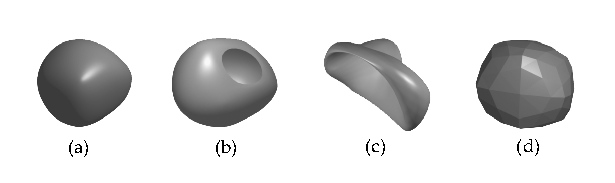
\epsfig{file=chapters/Curvature/s1234, width=130mm}
\end{center}
\vspace{-10pt}
\caption{(a) Closed, simple, smooth surface. (b) Not closed. (c) Not simple. (d) Not smooth.}
\label{fig:curvature-surfaces}
\end{figure}
%+++++++++++++++++++++++++++++++++++++++++

Example (a) in Figure~\ref{fig:curvature-surfaces} is a closed, simple surface. Surface (b) has a hole cut in it, so is not closed. Surface (c) can be thought of as having started out like surface (a), but with one side pushed back through the opposite side. So, surface (c), with its self intersection, is not simple, i.e. $\mathbf{p}(u_1,v_1) = \mathbf{p}(u_2,v_2)$ for some $(u_1,v_1) \ne (u_2,v_2)$.\\

A surface is called \emph{smooth} if the function $\mathbf{p}(u,v)$ is continuously differentiable. We define differentiability at the points $\mathbf{p}(u_{min},v)$ by considering a \emph{shifted} parameterization with $(u_{min}-\delta) \le u < (u_{max}-\delta)$ for some $\delta > 0$, thus extending the domain of the function $\mathbf{p}(u,v)$, such that $\mathbf{p}(u_{min}-\varepsilon,v) = \mathbf{p}(u_{max}-\varepsilon,v)$ whenever $0 < \varepsilon \le \delta$. We define differentiability at the points $\mathbf{p}(u,v_{min})$ similarly. Surface (d) in Figure~\ref{fig:curvature-surfaces}, composed of triangle facets, is not smooth where the facets meet.\\

A surface contains families of curves associated with its parameterization variables. Consider the family of curves given by
\begin{equation}
A_v = \left\{ \mathbf{p}(u,v) =
\left[
\begin{array}{c}
x(u,v) \\
y(u,v) \\
z(u,v)
\end{array}
\right]
:
u_{min} \le u < u_{max}\\
\right\}
\end{equation}
for some finite set of discrete fixed values of $v$ such that $v_{min} \le v < v_{max}$. Families given by $B_u$, with a fixed set of values of $u$, can be constructed similarly. Each point on a surface is contained in two \emph{parameterization curves}, one from each of the possible families $A_u$ and $B_v$.\\

Of course, for each curve in the families $A_u$ and $B_v$,  \emph{parameterization speed}, \emph{arc-length}, \emph{regularity}, \emph{singular points}, and \emph{tangent lines} are defined as in Section~\ref{sec:curvature-curves}.\\

\emph{By default, in this book, when we refer to a surface, we mean a smooth closed simple surface which does not contain any singular points.}\\

We define a (closed) \emph{surface patch} as any subset of a surface where that subset is parameterized by $u$ and $v$ where $a \le u \le b$ with $u_{min} \le a < b < u_{max}$, and $c \le v \le d$ with $v_{min} \le c < d < v_{max}$. Surface patches that include points given $\mathbf{p}(u_{min},v)$ and $\mathbf{p}(u,v_{min})$ can be constructed using a shift in parameterization as given in the previous discussion of differentiabily.\\

The \emph{area} of a surface patch is given by the following:
\begin{equation}
\int_{a}^{b} \int_{c}^{d} s(u,v)\, dv du
\end{equation}

Note that surface patch area is independent of the particular surface parameterization that is used.\\

%+++++++++++++++++++++++++++++++++++++++++
\begin{figure}[!t]
\begin{center}
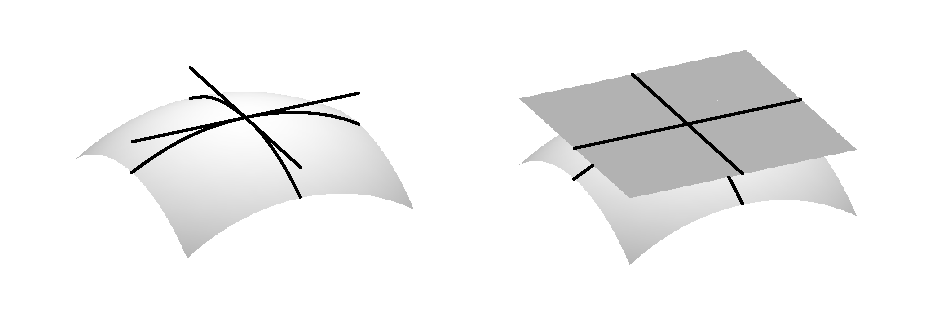
\epsfig{file=chapters/Curvature/tangent_plane, height=30mm}
\end{center}
\vspace{-20pt}
\caption{Parameterization curves and tangent lines on the left, the tangent plane on the right.}
\label{fig:curvature-tangent-plane}
\end{figure}
%+++++++++++++++++++++++++++++++++++++++++

Consider a point in a surface, and the two tangent lines associated, one each, with the two parameterization curves at that point as shown, for example, in Figure~\ref{fig:curvature-tangent-plane}. The unique plane which includes these two tangent lines is called the \emph{surface tangent plane}. Note that, for any given parameterization, the two tangent lines are not necessarily orthogonal to each other.\\

In general, a plane can be specified as the set of points
\begin{equation}
\label{eq:curvature-plane}
P = \left\{
\mathbf{p} : (\mathbf{p}-\mathbf{p}_0) \cdot \mathbf{\hat{n}} = 0
\right\}
\end{equation}
where the reference point $\mathbf{p}_0$ can be any point on the plane (one of an infinite number of possibilities) and the \emph{normal direction vector} $\hat{\mathbf{n}}$, could just as well be $- \hat{\mathbf{n}}$ (one of exactly two possibilities).\\

In the specific case of a surface tangent plane, a normal direction vector can be calculated simply as
\begin{equation}
\mathbf{\hat{n}} = \mathbf{\hat{t}_1} \times \mathbf{\hat{t}_2}
\end{equation}
where $\mathbf{\hat{t}_1}$ and $\mathbf{\hat{t}_2}$ are surface tangent line directions.\\

Once we have a surface tangent plane, we can construct a surface tangent line in any direction orthogonal to the tangent plane normal direction. We are thus not limited to the parameterization directions when considering surface tangent lines.\\

%------------- subsection ----------------
\subsection{Surface Curvature and Solid Regions}
\label{sec:curvature-surfaces}
%+++++++++++++++++++++++++++++++++++++++++
\begin{figure}[!t]
\begin{center}
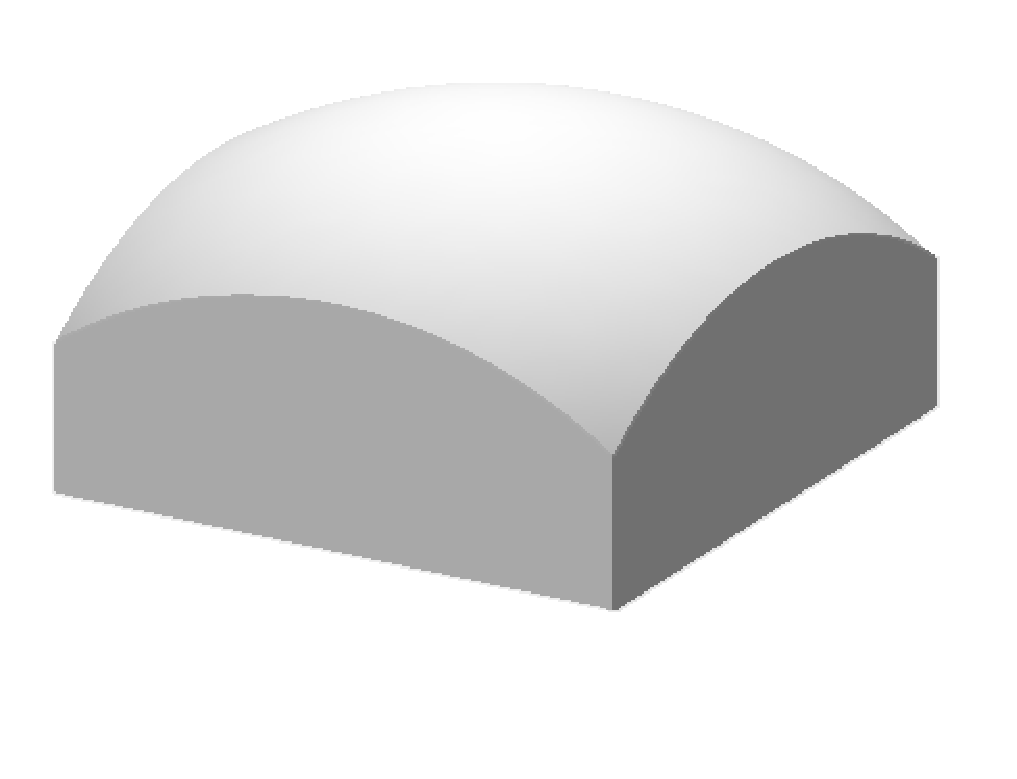
\epsfig{file=chapters/Curvature/surface_patch, height=25mm}
\end{center}
\vspace{-20pt}
\caption{Surface patch with a portion of its associated interior region.}
\label{fig:curvature-surface-patch}
\end{figure}
%+++++++++++++++++++++++++++++++++++++++++

A closed simple surface separates $\mathbb{R}^3$ into two solid regions: a bounded 
\emph{interior} and an unbounded \emph{exterior}\footnote{This is an example of a 
separation theorem. Separation theorems are important in topology, and have a 
rich history that dates back to \cite{Jordan_1887_CAP} and \cite{Veblen_1905_TPC}.}.  Figure~\ref{fig:curvature-surface-patch} 
shows a surface patch, with a portion of its associated interior region shaded.\\

In this work, we associate a (closed simple) surface, as well as each of its surface patches, with its interior region.\\

We build up to a definition of the \emph{surface normal vector} with some preliminaries.

\begin{definition}
The \emph{$\varepsilon$-neighborhood} of a point $\mathbf{p}$ in $\mathbb{R}^3$ is the open sphere of all points whose distance to $\mathbf{p}$ is less than $\varepsilon$.
\end{definition}

A \emph{ray} is the (half-line) set of points given by
\begin{equation}
\label{eq:curvature-ray}
R = \left\{ \mathbf{p}(t) =
\mathbf{p}_0 + \mathbf{\hat{r}} \, t
:
0 \le t < +\infty
\right\}
\end{equation}
where $\mathbf{p}_0$ is the ray starting point and $\mathbf{\hat{r}}$ is the (unit length) ray direction vector.\\

%+++++++++++++++++++++++++++++++++++++++++
\begin{figure}[!t]
\begin{center}
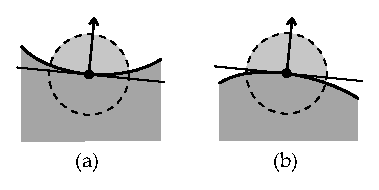
\epsfig{file=chapters/Curvature/surface_normal, height=30mm}
\end{center}
\vspace{-10pt}
\caption{Surface patch cross-sections with $\varepsilon$-neighborhood, tangent plane, and the exterior pointing normal.}
\label{fig:curvature-surface-normal}
\end{figure}
%+++++++++++++++++++++++++++++++++++++++++

Consider a point $\mathbf{p}$ on a surface, the tangent plane at that point, and the rays associated with the two possible tangent plane normal vectors. One of those normal vectors is \emph{exterior pointing} in that, for its associated ray, there exists an $\varepsilon$-neighborhood of \emph{$\mathbf{p}$} such that, within that $\varepsilon$-neighborhood, all of the points of the ray, except for \emph{$\mathbf{p}$} itself, are part of the surface exterior region. See Figure~\ref{fig:curvature-surface-normal} for examples.

\begin{definition}
The \emph{surface normal vector} at a point in a surface is the exterior pointing tangent plane normal vector at that point.
\end{definition}

%+++++++++++++++++++++++++++++++++++++++++
\begin{figure}[!t]
\begin{center}
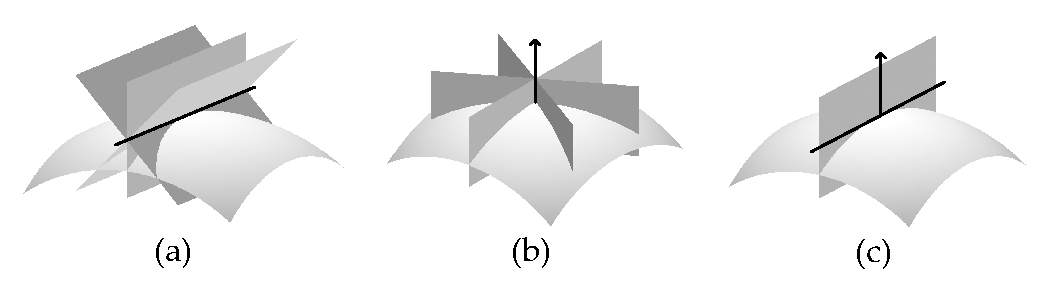
\epsfig{file=chapters/Curvature/cutting_planes, height=30mm}
\end{center}
\vspace{-10pt}
\caption{Cutting planes: (a) aligned with a surface tangent line, (b) aligned with the surface normal, (c) the unique plane aligned with both a surface tangent line and the surface normal.}
\label{fig:curvature-cutting-planes}
\end{figure}
%+++++++++++++++++++++++++++++++++++++++++

A surface \emph{cutting plane} through the point $\mathbf{p}$ in a surface, is any plane, other than the tangent plane, containing $\mathbf{p}$. A \emph{normal cutting plane} through a point in a surface, is a surface cutting plane that includes the surface normal at that point. Note that there is a unique normal cutting plane that includes any given surface tangent line. Figure~\ref{fig:curvature-cutting-planes} illustrates examples of cutting planes.\\

%+++++++++++++++++++++++++++++++++++++++++
\begin{figure}[!t]
\begin{center}
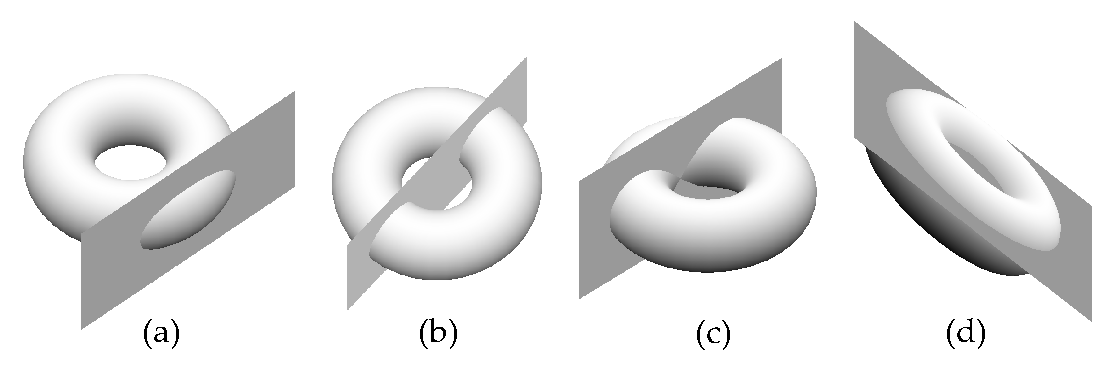
\epsfig{file=chapters/Curvature/plane_curves, height=38mm}
\end{center}
\vspace{-10pt}
\caption{Cutting plane intersections: (a) single curve, (b) two curves, (c) self-intersecting curve, (d) concentric curves.}
\label{fig:curvature-plane-curves}
\end{figure}
%+++++++++++++++++++++++++++++++++++++++++

The intersection of a surface and a surface cutting plane associated with a point in the
surface, is (locally) a smooth simple arc which includes that point. Globally, the
intersection may include singular points, additional curves, and the curves may
self-intersect. Examples are shown in Figure~\ref{fig:curvature-plane-curves}. Note that
in Figure~\ref{fig:curvature-plane-curves} (d), the surface interior region is an annulus
which lies between two concentric intersection curves.

\begin{definition}
The \emph{normal curvature} $\kappa_n$ at a point in a surface, along the \emph{direction} of
a surface tangent line, is the (signed) curvature of the curve which is the intersection of
that surface and the normal cutting plane aligned with the tangent line at that point.
\end{definition}

With this definition, curvature polarity is assigned based on surface interior points
within the cutting plane subset thought of as planar curve interior points.

\begin{definition}
The \emph{principal curvatures}, $\kappa_1$ and $\kappa_2$, at a point in a surface are the
respective maximum and minimum values of the normal curvature at that point.
\end{definition}

The following Theorem is a fundamental result from differential geometry and can be found in \cite{doCarmo_1976_DGCS}.
\begin{theorem}
\label{theorem:curvature-normal-curvature}
The relationship between normal curvature and the principal curvatures is given by
\begin{equation}
\label{eq:curvature-normal-curvature}
\kappa_n = \kappa_1 \cos ^2 \theta + \kappa_2 \sin ^2 \theta
\end{equation}
where $\theta$ is the angle between an arbitrary normal curvature ($\kappa_n$) cutting plane (or direction) and the maximum curvature ($\kappa_1$) cutting plane (or direction).\\
\end{theorem}

Theorem~\ref{theorem:curvature-normal-curvature} implies that \emph{the principal curvature cutting planes (and directions) are orthogonal to each other}. (This can be verified by setting $\theta$ in Equation~(\ref{eq:curvature-normal-curvature}) to the value $0$ and then to the value $\pm \pi / 2$.)\\

We are now in a position to define two frequently used standard surface curvature measures.

\begin{definition}
The \emph{mean curvature} is defined as
\begin{equation}
H = \frac{\kappa_1 + \kappa_2}{2}
\label{eq:curvature-def-mean}
\end{equation}
\end{definition}

\begin{definition}
The \emph{Gaussian curvature} is defined as
\begin{equation}
K = \kappa_1 \kappa_2
\label{eq:curvature-def-gaussian}
\end{equation}
\end{definition}

Often, in practice, as we see later in this book, normal curvatures can be directly 
calculated, but the principal curvatures cannot. Fortunately, using the following 
well-known theorem, \emph{mean curvature can be calculated without knowing the principal 
curvatures}.

\begin{theorem}(Two-Cut Mean Curvature)
\label{theorem:curvature-2-cut}
Using any two normal cutting planes which are orthogonal to each other, the mean curvature at a point on a surface is given by
\begin{equation}
H = \frac{\kappa_{n_1} + \kappa_{n_2}}{2}
\end{equation}
where $\kappa_{n_1}$ and $\kappa_{n_2}$ are normal curvatures associated with those cutting planes.\\
\end{theorem}

\begin{proof}
Consider the normal curvatures, $\kappa_{n_1}$ and $\kappa_{n_2}$, associated with two 
orthogonal normal cutting planes, with the first cutting plane oriented at an arbitrary 
angle $\alpha$ with the maximum principal curvature direction, and the second cutting plane 
oriented at the angle $\alpha + \pi/2$. From Equation~(\ref{eq:curvature-normal-curvature}) 
we have that

\begin{equation}
\kappa_{n_1} = \kappa_1 \cos ^2 \alpha + \kappa_2 \sin ^2 \alpha
\label{eq:curvature-kn1}
\end{equation}
and
\begin{align}
\kappa_{n_2} &= \kappa_1 \bigr( \cos (\alpha + \pi/2) \bigl) ^2  + \kappa_2 \bigl( \sin (\alpha + \pi/2) \bigr) ^2 \\
&= \kappa_1 (-\sin \alpha)^2 + \kappa_2 (\cos \alpha)^2\\
&= \kappa_1 \sin^2 \alpha + \kappa_2 \cos^2 \alpha
\label{eq:curvature-kn2}
\end{align}
Combining Equations~(\ref{eq:curvature-kn1})~and~(\ref{eq:curvature-kn2}), we have that
\begin{align}
\kappa_{n_1} + \kappa_{n_2}
&=
(\kappa_1 \sin^2 \alpha + \kappa_2 \cos^2 \alpha)
+ (\kappa_1 \cos ^2 \alpha + \kappa_2 \sin ^2 \alpha)\\
&=
\kappa_1 \sin^2 \alpha + \kappa_1 \cos ^2 \alpha
+ \kappa_2 \sin ^2 \alpha + \kappa_2 \cos^2 \alpha\\
&=
\kappa_1 (\sin^2 \alpha + \cos ^2 \alpha)
+ \kappa_2 (\sin ^2 \alpha + \cos^2 \alpha)\\
&= \kappa_1 + \kappa_2\\
\end{align}
It follows that
\begin{align}
\frac{\kappa_{n_1} + \kappa_{n_2}}{2} &= \frac{\kappa_1 + \kappa_2}{2} = H
\end{align}

This proves the theorem.\qed
\end{proof}

\vspace{20pt}
In this book, we generalize the two-cut mean curvature theorem to \emph{n-cuts}. But first, 
some preliminary results are required.

\begin{lemma}
\label{lemma:curvature-angle-sum}
For $n \ge 2$, and any non-zero integer $c$ such that $n$ does not divide $c$,
\begin{align}
\sum_{m=0}^{n-1} \cos \bigl(2c \pi \, m / n \bigr) =
\sum_{m=0}^{n-1} \sin \bigl(2c \pi \, m / n \bigr) &= 0
\end{align}
\end{lemma}
\begin{proof}

Recall the following identity for the partial sums of a geometric series where $z$ is a 
complex number (not equal to one):
\begin{equation}
z^0 + z^1 + z^2 + \dots + z^{n-1} = \frac{z^n - 1}{z - 1}
\end{equation}
Consider the following summation, where $n \ge 2$, and $c$ is a non-zero integer such that $n$ does not divide $c$:
\begin{align}
\sum_{m=0}^{n-1} e^{i 2c\pi \,m/n}
&= \bigl( e^{i 2c \pi /n} \bigr)^0
+ \bigl( e^{i 2c \pi /n} \bigr)^1
+ \bigl( e^{i 2c \pi /n} \bigr)^2
+ \dots
+ \bigl( e^{i 2c \pi /n} \bigr)^{n-1}\\
&= \frac{\bigl( e^{i 2c \pi /n} \bigr)^n - 1}{e^{i 2c \pi /n} - 1}\\
&= \frac{e^{i 2c \pi} - 1}{e^{i 2c \pi /n} - 1}\\
&= \frac{1 - 1}{e^{i 2c \pi /n} - 1}\\
\label{eq:curvature-mn2}
&= \frac{0}{e^{i 2c \pi /n} - 1} = 0
\end{align}
But we also have that
\begin{align}
\sum_{m=0}^{n-1} e^{i 2c\pi \,m/n}
&= \sum_{m=0}^{n-1} \Bigl( \cos \bigl(2c \pi \, m / n \bigr)
+ i \sin \bigl(2c \pi \, m / n \bigr) \Bigr)\\
\label{eq:curvature-mn1}
&= \sum_{m=0}^{n-1} \cos \bigl(2c \pi \, m / n \bigr)
+ i \sum_{m=0}^{n-1} \sin \bigl(2c \pi \, m / n \bigr)
\end{align}
Taking Equations~(\ref{eq:curvature-mn2}) and (\ref{eq:curvature-mn1}) together gives
\begin{align}
\sum_{m=0}^{n-1} \cos \bigl(2c \pi \, m / n \bigr)
+ i\sum_{m=0}^{n-1} \sin \bigl(2c \pi \, m / n \bigr) = 0
\end{align}
which implies that
\begin{align}
\sum_{m=0}^{n-1} \cos \bigl(2c \pi \, m / n \bigr) =
\sum_{m=0}^{n-1} \sin \bigl(2c \pi \, m / n \bigr) = 0
\end{align}


This proves the lemma.\qed
\end{proof}

\begin{lemma}
\label{lemma:curvature-angle-squared-sum}
For $n > 2$,
\begin{equation}
\sum_{m=0}^{n-1} \cos ^2 \bigl(2\pi \, m / n \bigr) =
\sum_{m=0}^{n-1} \sin ^2 \bigl(2\pi \, m / n \bigr)
= \frac{n}{2}
\end{equation}
\end{lemma}
\begin{proof}
\begin{align}
\sum_{m=0}^{n-1} \cos ^2 \bigl(2\pi \, m / n \bigr) &=
\sum_{m=0}^{n-1} \frac{1 + \cos (4\pi \, m / n )}{2}\\
&= \sum_{m=0}^{n-1} \frac{1}{2}
\, + \, \frac{1}{2} \sum_{m=0}^{n-1} \cos (4\pi \, m / n )\\
&= \frac{n}{2} \, + \, \frac{1}{2} \Bigl( 0 \Bigr) = \frac{n}{2}
\end{align}
\begin{align}
\sum_{m=0}^{n-1} \sin ^2 \bigl(2\pi \, m / n \bigr) &=
\sum_{m=0}^{n-1} \frac{1 - \cos (4\pi \, m / n )}{2}\\
&= \sum_{m=0}^{n-1} \frac{1}{2}
\, - \, \frac{1}{2} \sum_{m=0}^{n-1} \cos (4\pi \, m / n )\\
&= \frac{n}{2} \, - \, \frac{1}{2} \Bigl( 0 \Bigr) = \frac{n}{2}
\end{align}


This proves the lemma.\qed
\end{proof}

\begin{theorem}(n-Cut Mean Curvature)
\label{theorem:curvture-n-cut}
Using any $n > 2$ equally spaced (by angle) normal cutting planes, the mean curvature at a point on a surface is the mean of the associated normal curvatures.
\end{theorem}
This can be written as:
\begin{equation}
H = \frac{1}{n} \sum_{m=0}^{n-1} \kappa_{n_m}
\end{equation}
where $\kappa_{n_m}$ is the normal curvature associated with the $(m+1)$-th cutting plane.\\

\begin{proof}
Consider $n > 2$ equally spaced normal cutting planes, with an arbitrary constant angle $\alpha$ between the first cutting plane and the maximum principal curvature direction.\\

Let $\beta = 2\pi \, m / n$. From Equation~(\ref{eq:curvature-normal-curvature}) we have:
\begin{equation}
\label{eq:curvature-sum}
\sum_{m=0}^{n-1} \kappa_{n_m}
= \kappa_1 \sum_{m=0}^{n-1}\cos ^2 \bigl(\alpha + \beta \bigr)
+ \kappa_2 \sum_{m=0}^{n-1} \sin ^2 \bigl(\alpha + \beta \bigr)
\end{equation}

Consider the $\kappa_1$ summation term from Equation~(\ref{eq:curvature-sum}) :
\begin{align}
\sum_{m=0}^{n-1} \cos ^2 &( \alpha + \beta )
= \sum_{m=0}^{n-1} ( \cos \alpha \cos \beta - \sin \alpha \sin \beta ) ^2\\
&= \sum_{m=0}^{n-1} ( \cos^2 \alpha \cos^2 \beta
- 2 \cos \alpha \sin \alpha \cos \beta \sin \beta
+ \sin^2 \alpha \sin^2 \beta)\\
&= \cos^2 \alpha \sum_{m=0}^{n-1} \cos^2 \beta
- \cos \alpha \sin \alpha \sum_{m=0}^{n-1} \sin 2 \beta
+ \sin^2 \alpha \sum_{m=0}^{n-1} \sin^2 \beta\\
\label{eq:curvature-sum-k1}
&= ( \cos^2 \alpha ) \Bigl( \frac{n}{2} \Bigr)
- (\cos \alpha \sin \alpha) \Bigl( 0 \Bigr)
+ ( \sin^2 \alpha ) \Bigl( \frac{n}{2} \Bigr)\\
&= ( \cos^2 \alpha + sin^2 \alpha) \,\frac{n}{2}\\
&= \frac{n}{2}
\end{align}

Note that Equation~(\ref{eq:curvature-sum-k1}) employs Lemmas~\ref{lemma:curvature-angle-sum} and \ref{lemma:curvature-angle-squared-sum}.\\

Consider the $\kappa_2$ summation term from Equation~(\ref{eq:curvature-sum}) :
\begin{align}
\sum_{m=0}^{n-1} \sin ^2 &( \alpha + \beta )
= \sum_{m=0}^{n-1} ( \sin \alpha \cos \beta + \cos \alpha \sin \beta ) ^2\\
&= \sum_{m=0}^{n-1} ( \sin^2 \alpha \cos^2 \beta
+ 2 \cos \alpha \sin \alpha \cos \beta \sin \beta
+ \cos^2 \alpha \sin^2 \beta)\\
&= \sin^2 \alpha \sum_{m=0}^{n-1} \cos^2 \beta
+ \cos \alpha \sin \alpha \sum_{m=0}^{n-1} \sin 2 \beta
+ \cos^2 \alpha \sum_{m=0}^{n-1} \sin^2 \beta\\
&= ( \sin^2 \alpha ) \Bigl( \frac{n}{2} \Bigr)
+ (\cos \alpha \sin \alpha) \Bigl( 0 \Bigr)
+ ( \cos^2 \alpha ) \Bigl( \frac{n}{2} \Bigr)\\
&= ( \sin^2 \alpha + \cos^2 \alpha) \,\frac{n}{2}\\
&= \frac{n}{2}
\end{align}

Substituting these results back into Equation~(\ref{eq:curvature-sum}) gives:
\begin{align}
\sum_{m=0}^{n-1} \kappa_{n_m}
&= \kappa_1 \Bigl( \frac{n}{2} \Bigr)
+ \kappa_2 \Bigl( \frac{n}{2} \Bigr)\\
&= n \Bigl( \frac{\kappa_1 + \kappa_2}{2} \Bigr)\\
\frac{1}{n} \sum_{m=0}^{n-1} \kappa_{n_m} &= \frac{\kappa_1 + \kappa_2}{2} = H
\end{align}

This proves the theorem.\qed
\end{proof}

%------------- subsection ----------------
\subsection{Surface Curvature Computation}
In our discussion of surface curvature so far, we have taken a geometric view in the sense 
that we have used cutting planes in defining normal curvature and, hence, the principal 
curvatures. (The motivation for this approach becomes clear later in this book when we 
consider \emph{digitized surfaces}.) Alternatively, given an explicit surface 
parameterization (i.e. a set of parametric equations), it is also possible to take an 
analytical approach to surface curvature and its computation.\\

To this end, a number of standard working variables are defined in differential geometry.
Given a surface parameterization $\mathbf{p}(u,v)$, the \emph{first fundamental form} variables are
\begin{align}
E &= \mathbf{p}_u \cdot \mathbf{p}_u\\
F &= \mathbf{p}_u \cdot \mathbf{p}_v\\
G &= \mathbf{p}_v \cdot \mathbf{p}_v
\end{align}
and the \emph{second fundamental form} variables are
\begin{align}
l &= \mathbf{\hat{n}} \cdot \mathbf{p}_{uu}\\
m &= \mathbf{\hat{n}} \cdot \mathbf{p}_{uv}\\
n &= \mathbf{\hat{n}} \cdot \mathbf{p}_{vv}
\end{align}
where we have used the notational convention, for example, $\mathbf{p}_u = \partial \mathbf{p}(u,v) / \partial u$ and $\mathbf{p}_{uu} = \partial \mathbf{p}_u / \partial u$.\\

The \emph{Weingarten matrix} $L$ is defined as the unique $2 \! \times \! 2$ matrix, such that, for every point in a surface, we have
\begin{equation}
\left[
\begin{array}{cc}
\mathbf{\hat{n}}_u & \mathbf{\hat{n}}_v
\end{array}
\right]
=
\left[
\begin{array}{cc}
\mathbf{p}_u & \mathbf{p}_v
\end{array}
\right]
L
\end{equation}
where
\begin{equation}
\mathbf{\hat{n}} =
\frac{\mathbf{p}_u \times \mathbf{p}_v}{|| \mathbf{p}_u \times \mathbf{p}_v ||}
\end{equation}\\

Remarkably, the eigenvalues of the matrix $L$ give the principal curvatures (as $-\kappa_1$ and $-\kappa_2$), and the eigenvectors of $L$ are the \emph{principal curvature directions}. Note that a curvature direction corresponds to the direction of the surface tangent line that is coincident with the associated normal curvature cutting plane.\\

One of the most important theoretical results in differential geometry is an explicit formulation for the Weingarten matrix in terms of the first and second fundamental form variables:
\begin{equation}
L = \frac{1}{EG - F^2}
\left[
\begin{array}{cc}
Fm - Gl & Fn - Gm\\
Fl - Em & Fm - En
\end{array}
\right]
\label{eq:curvature-weingarten}
\end{equation}
It is well worth noting that, with the assistance of modern symbolic math computer software
that can compute eigenvalues and eigenvectors, the Weingarten matrix can be put to
practical use, giving explicit symbolic formulations for the principal curvatures and the
principal curvature directions.\\

Additionally (or alternatively), mean curvature can be given in terms of of the first and second fundamental form variables as
\begin{equation}
H = \frac{En + Gl - 2Fm}{2 (EG - F^2)}
\label{eq:curvature-mean}
\end{equation}
and Gaussian curvature is given as
\begin{equation}
K = \frac{ln - m^2}{EG - F^2}
\label{eq:curvature-gaussian}
\end{equation}
And then, using the definitions of mean and Gaussian curvature given in Equations~(\ref{eq:curvature-def-mean}) and (\ref{eq:curvature-def-mean}), we can extract the principal curvatures as
\begin{equation}
\kappa_1 = H + \sqrt{H^2 - K}
\label{eq:curvature-k1}
\end{equation}
and
\begin{equation}
\kappa_2 = H - \sqrt{H^2 - K}
\label{eq:curvature-k2}
\end{equation}

For derivations of Equations (\ref{eq:curvature-weingarten}), (\ref{eq:curvature-mean}) and(\ref{eq:curvature-gaussian}) see, for example \cite{Davies_1996_CGCS} or \cite{doCarmo_1976_DGCS}.\\

%---------------- section ----------------
\section{Scale Invariant Curvature}
\label{sec:curvature-invariant}
It is generally useful to seek \emph{invariant} properties when characterizing 3D objects. 
At a minimum, translation and rotation invariant characterization is desired as clearly 
neither of these transformations alters the essential shape property of an object. Surface 
curvature, a rotation and translation invariant property, meets this requirement.\\

Any characterization that is additionally \emph{scaling invariant} enables determining the equivalence of shapes independent of size. Perhaps not so obvious, practically speaking, this scale invariance would also enable the use of uncalibrated measurement units in 3D digitization (e.g. scanning).\\

\emph{None of the curvature measures defined so far in this chapter are scale invariant.}\\

In this section we introduce a new scale invariant curvature measure, \emph{similarity curvature}. We also define a similarity curvature space which consists of the set of all possible similarity curvature values.\\

%------------- subsection ----------------
\subsection{Geometric Invariants}
As previously noted, with existing surface curvature definitions, we already have translation and rotation invariance. What we now seek is scaling invariance. Note that shape characterization based on moments has been studied following work by \cite{Hu_1962_VPRMI}, with varying emphasis on invariance with respect to translation, rotation, reflection, or scaling.\\

Related work \cite{Sapiro_2001_GPDEIA}, among other things, generalizes and extends the invariance concepts contained in affine differential geometry. Affine invariance is stronger than what we seek in that it includes, for example, squash and stretch transformations.\\

A number of authors touch on scaling invariant properties in their exploration of multi-scale properties. For example, in \cite{Mokhtarian_2003_CSSR}, firstly surface feature points such as maximum curvature locations are identified. Then triples of feature points are combined using a geometric hashing algorithm in a way that is scaling invariant. Hash tables for various objects of interest are statistically compared to check for similarity matches between different objects.

%------------- subsection ----------------
\subsection{A Scale Invariant Curvature Measure}
\label{sec:curvature-similarity}
In this section, we present a scale invariant curvature measure that can be assigned \emph{at every point on a surface}. We keep in mind that any definition of scale invariant surface curvature must be related to geometric similarity in which it is well-known that 1) angles are preserved and 2) ratios of lengths are preserved.\\

We start with some definitions.

\begin{definition}
\label{def:curvature-similarity1}
Given principal curvatures $\kappa_1$ and $\kappa_2$, the curvature ratio $\kappa_3$ is defined as
\begin{equation*}
\kappa_3 = \frac{\textup{min}(|\kappa_1|,|\kappa_2|)}{\textup{max}(|\kappa_1|,|\kappa_2|)}
\end{equation*}
\end{definition}

In the case when $\kappa_1$ and $\kappa_2$ are both equal to zero, $\kappa_3$ is defined as being equal to zero.
Note that $0 \le \kappa_3 \le 1$.\\

\begin{definition}
\label{def:curvature-similarity2}
The similarity curvature $R$ at a point in a surface is defined as
\begin{equation}
R =
\begin{cases}
(\kappa_3,0) & \textup{ if signs of $\kappa_1$ and $\kappa_2$ are both positive,} \\
(-\kappa_3,0) & \textup{ if signs of $\kappa_1$ and $\kappa_2$ are both negative,} \\
(0,\kappa_3) & \textup{ if signs of $\kappa_1$ and $\kappa_2$ differ, and } \kappa_1 \ge |\kappa_2|, \\
(0,-\kappa_3) & \textup{ if signs of $\kappa_1$ and $\kappa_2$ differ, and } \kappa_1 < |\kappa_2|. \\
\end{cases}
\label{eq:similarity-curvature}
\end{equation}
\end{definition}

Note that $R \in \mathbb R^2$.

\begin{theorem}
For every closed, simple, smooth surface, the curvature measure $R$ is (positive) scaling invariant.
\end{theorem}
\begin{proof}
Consider a point on a surface and any associated normal curvature $\kappa$, as well as the resultant normal curvature $\kappa^\prime$ after scaling the surface by a factor $s$. Since, by definition, $\kappa=d\alpha / dl$, and scaling alters length but not angle, we have $\kappa^\prime = \kappa / s$.\\ Therefore, after scaling, both of the principal curvatures change by the same factor, and the ratio of the principal curvatures is unchanged. Also, neither the signs, nor the relative magnitudes of the principal curvatures are changed by scaling.\\

This proves the theorem.\qed
\end{proof}
\vspace{20pt}

Henceforth, we will refer to the curvature measure $R$ as the \emph{similarity curvature}.

%------------- subsection ----------------
\subsection{The Similarity Curvature Space}
\label{sec:curvature-similarity-space}
Since the set of all possible values of the similarity curvature $R$ is a subset of $\mathbb R^2$, it is natural to consider a two-dimensional plot representation. Also recall, from differential geometry, that all surface patches on continuous smooth surfaces are locally either elliptic, hyperbolic (saddle-like), parabolic or planar.\\

%+++++++++++++++++++++++++++++++++++++++++
\begin{figure}[!t]
\begin{center}
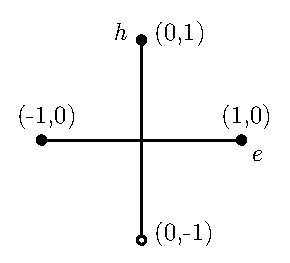
\epsfig{file=chapters/Curvature/eh_plot1, height=35mm}
\end{center}
\vspace{-10pt}
\caption{$eh$-plot space for similarity curvature.}
\label{fig:curvature-eh-plot1}
\end{figure}
%+++++++++++++++++++++++++++++++++++++++++

We introduce the similarity curvature plot template in Figure~\ref{fig:curvature-eh-plot1}. The horizontal $e$-axis is for curvature values at locally elliptic surface points. The vertical $h$-axis is for curvature values at locally hyperbolic surface points. Both parabolic and planar surface points have similarity curvature value $(0,0)$ and are thus plotted at the origin. Plotted similarity curvature values will never be off the axes.\\

When considering examples, it is clear that the similarity curvature at every point on all spheres is constant and equal to $(1,0)$. The similarity curvature on every planar surface, every cylinder and every cone is constant\footnote{Excluding the cylinder and cone edges and the cone apex.} and equal to $(0,0)$. Note that this is exactly where the Gaussian curvature is equal to zero.\\

Continuous motion through points on a smooth surface, taking the similarity curvature at each point, results in a related continuous motion in the similarity plot space. We observe, for example, that it is not possible to traverse from similarity curvature (-1,0) to similarity curvature (1,0) without going through similarity curvature (0,0).\\

However, it is possible to traverse from (0,1) directly to (0,-1). This can be described by 
saying that the $h$-axis \emph{wraps around}. An example where this wrapping occurs is 
given later.\\

%---------------- section ----------------
\section{Curvature Visualization}
\label{sec:curvature-visualization}
We can visualize surface curvature magnitude in illustrations by coloring or grey-scale shading the surface points. With this visualization technique, we can see the patterns of curvature variation across a surface. The goal in this section is to gain insight into the nature of, and differences between, curvature measures.\\

Given an explicit surface parameterization, Equations~(\ref{eq:curvature-mean}) and (\ref{eq:curvature-gaussian}) can be used respectively to calculate exact values for mean and Gaussian curvature.\\

%+++++++++++++++++++++++++++++++++++++++++
\begin{figure}[!t]
\begin{center}
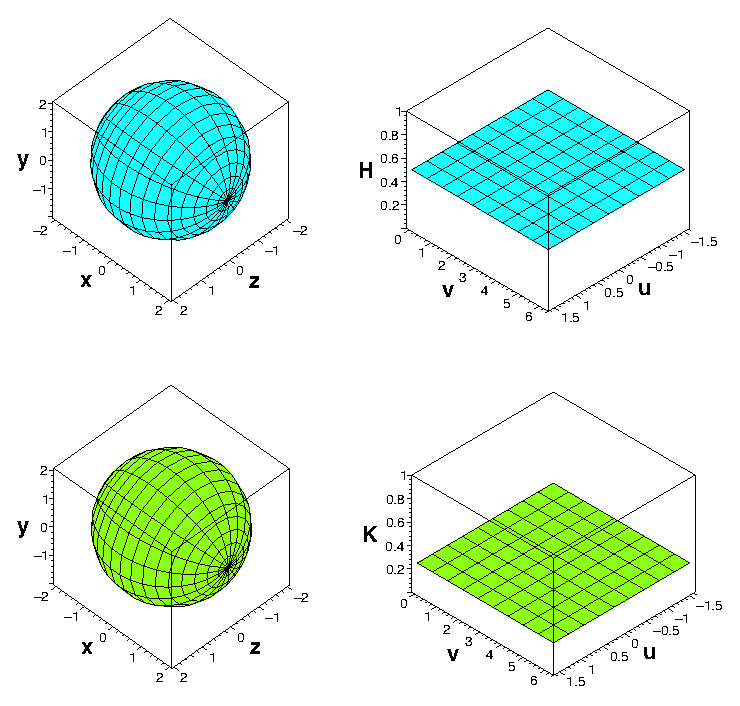
\epsfig{file=chapters/Curvature/sphere_HK, height=110mm}
\end{center}
\vspace{-10pt}
\caption{Mean (top) and Gaussian (bottom) curvature for a parameterized sphere of radius 2.}
\label{fig:curvature-sphere-HK}
\end{figure}
%+++++++++++++++++++++++++++++++++++++++++

Consider the following sphere parameterization:
\begin{equation}
S = \left\{ \mathbf{p}(u,v) =
\left[
\begin{array}{c}
r \sin u \\
r \cos u \cos v\\
r \cos u \sin v
\end{array}
\right]
:
(-\pi/2 \le u < \pi/2) \, \wedge \, (0 \le v < 2\pi)
\right\}
\end{equation}\\

Figure~\ref{fig:curvature-sphere-HK} shows results for this sphere parameterization when the radius $r=2$. The color coded sphere object itself is shown on the left, and curvature versus parameterization is shown on the right. For spheres, in general, both the mean curvature and the Gaussian curvature are always constant. For the sphere shown, the mean curvature is $1/2$ and the Gaussian curvature is $1/4$.\\

%+++++++++++++++++++++++++++++++++++++++++
\begin{figure}[!t]
\begin{center}
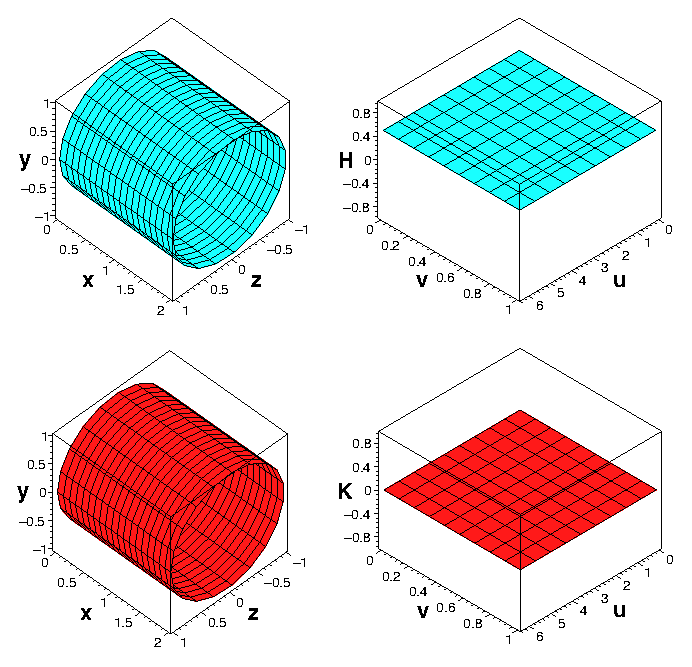
\epsfig{file=chapters/Curvature/cylinder_HK, height=110mm}
\end{center}
\vspace{-10pt}
\caption{Mean (top) and Gaussian (bottom) curvature for a parameterized cylinder of radius 1 and height 2.}
\label{fig:curvature-cylinder-HK}
\end{figure}
%+++++++++++++++++++++++++++++++++++++++++

Consider the following cylinder parameterization:
\begin{equation}
S = \left\{ \mathbf{p}(u,v) =
\left[
\begin{array}{c}
h v\\
r \sin u\\
r \cos u
\end{array}
\right]
:
(0 \le u < 2\pi) \, \wedge \, (0 \le v < 1)
\right\}
\end{equation}\\

Figure~\ref{fig:curvature-cylinder-HK} shows results for this cylinder parameterization when the radius $r=1$ and the height $h=2$. For cylinders, in general, both the mean curvature and the Gaussian curvature are always constant, as is the case for spheres. However, in contrast with spheres, all cylinders have Gaussian curvature zero. For the cylinder shown, the mean curvature is $1/2$.\\

%+++++++++++++++++++++++++++++++++++++++++
\begin{figure}[!t]
\begin{center}
\epsfig{file=chapters/Curvature/cone_HK, height=110mm}
\end{center}
\vspace{-10pt}
\caption{Mean (top) and Gaussian (bottom) curvature for a (truncated) parameterized cone having base radius $1/2$ and height 1.}
\label{fig:curvature-cone-HK}
\end{figure}
%+++++++++++++++++++++++++++++++++++++++++

Consider the following truncated cone parameterization:
\begin{equation}
S = \left\{ \mathbf{p}(u,v) =
\left[
\begin{array}{c}
h v\\
r (1-v) \sin u\\
r (1-v) \cos u
\end{array}
\right]
:
(0 \le u < 2\pi) \, \wedge \, (0 \le v < 0.8)
\right\}
\end{equation}\\

Figure~\ref{fig:curvature-cone-HK} shows results for this cone parameterization when the base radius $r=1/2$ and the height $h=1$, with the apex cut off at 0.8 times the height. As is the case for cylinders, all cones have Gaussian curvature zero. For the cylinder shown, the mean curvature is $1$ at the base, increasing to $4.5$ towards the apex.\\

%+++++++++++++++++++++++++++++++++++++++++
\begin{figure}[!t]
\begin{center}
\epsfig{file=chapters/Curvature/torus_HK, height=110mm}
\end{center}
\vspace{-10pt}
\caption{Mean (top) and Gaussian (bottom) curvature for a parameterized torus.}
\label{fig:curvature-torus-HK}
\end{figure}
%+++++++++++++++++++++++++++++++++++++++++

Consider the following torus parameterization:
\begin{equation}
S = \left\{ \mathbf{p}(u,v) =
\left[
\begin{array}{c}
(a + b \cos u ) \cos v \\
(a + b \cos u ) \sin v \\
b \sin u
\end{array}
\right]
:
(0 \le u < 2\pi) \, \wedge \, (0 \le v < 2\pi)
\right\}
\end{equation}\\

Figure~\ref{fig:curvature-torus-HK} shows results for this torus parameterization when radius $a=1$ and radius $b=1/3$. In this figure, the color range for each of the curvatures is separately set to span the range of curvature values. Thus, the range (and offset) of the color scale for each of the curvatures is not the same. However, with this color scale, the curvature visualizations for Gauassian and mean curvature appear almost identical. In this sense, at least for the given torus, the \emph{shape} of the curvatures is nearly the same.\\

Of course, for the given torus, the absolute values of the curvatures are clearly not the same. The mean curvatures are non-negative, while the Gaussian curvatures span both positive and negative values.\\

%+++++++++++++++++++++++++++++++++++++++++
\begin{figure}[!t]
\begin{center}
\epsfig{file=chapters/Curvature/ellipsoid_HK, height=110mm}
\end{center}
\vspace{-10pt}
\caption{Mean (top) and Gaussian (bottom) curvature for a parameterized ellipsoid.}
\label{fig:curvature-ellipsoid-HK}
\end{figure}
%+++++++++++++++++++++++++++++++++++++++++

Consider the following ellipsoid parameterization:
\begin{equation}
S = \left\{ \mathbf{p}(u,v) =
\left[
\begin{array}{c}
a \sin u \\
b \cos u \cos v\\
c \cos u \sin v
\end{array}
\right]
:
(-\pi/2 \le u < \pi/2) \, \wedge \, (0 \le v < 2\pi)
\right\}
\label{eq:curvature-ellipsoid}
\end{equation}\\

Figure~\ref{fig:curvature-ellipsoid-HK} shows results for this ellipsoid parameterization
when $a=\sqrt{3}$, $b=\sqrt{2}$, and $c=1$. In this figure, the color range for each of the
curvatures is separately set to span the range of curvature values. Thus, the range (and
offset) of the color coding scale for each of the curvatures is not the same. However, with
this color scale, as was the case for the torus, the curvature visualizations for Gaussian
and mean curvature appear similar. Again, the \emph{shape} of the curvatures is similar.\\

Interestingly, at least for the given ellipsoid, the actual values of the Gaussian and mean curvatures are similar as well.\\

For any given surface prameterization, Equations~(\ref{eq:curvature-mean}) and (\ref{eq:curvature-gaussian}) can also be used to develop explicit formulae for Gaussian and mean curvature respectively. However, performing the algebraic operations required to simplify these formulae can be rather tedious!\\

The resultant formula for Gaussian curvature of the ellipsoid given by Equation~(\ref{eq:curvature-ellipsoid}) is
\begin{equation}
K = \frac{a^2 b^2 c^2}
{(
b^2 c^2
- ((b^2- c^2) a^2 \cos^2v + b^2 (c^2 - a^2)) \cos^2u
)^2}
\end{equation}
and the resultant formula for mean curvature is
\begin{equation}
H =
\left( \frac{a b c }{2} \right)
\frac{
b^2 + c^2
+ (a^2 - c^2 + (c^2 - b^2) \cos^2v
) \cos^2u
}{(b^2 c^2
- ((b^2- c^2) a^2 \cos^2v + b^2 (c^2 - a^2)) \cos^2u
)^{3/2}}
\end{equation}\\

Using the same ellipsoid parameterization, we can also visualize an example of similarity curvature.\\

%+++++++++++++++++++++++++++++++++++++++++
\begin{figure}[!t]
\begin{center}
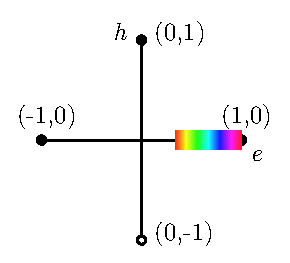
\epsfig{file=chapters/Curvature/eh_plotC1, height=35mm}
\end{center}
\vspace{-10pt}
\caption{EH-plot space color assignment for the ellipsoid example.}
\label{fig:curvature-eh-plotC1}
\end{figure}
%+++++++++++++++++++++++++++++++++++++++++

%+++++++++++++++++++++++++++++++++++++++++
\begin{figure}[!t]
\begin{center}
\epsfig{file=chapters/Curvature/ellipsoid_RX, height=110mm}
\end{center}
\vspace{-10pt}
\caption{Similarity curvature for a parameterized ellipsoid scaled at 1x (top) and 100x (bottom).}
\label{fig:curvature-ellipsoid-RX}
\end{figure}
%+++++++++++++++++++++++++++++++++++++++++

Figure~\ref{fig:curvature-ellipsoid-RX} shows results for this ellipsoid parameterization
when $a=\sqrt{3}$, $b=\sqrt{2}$, and $c=1$ at a 1x scale and a 100x scale. Note that, since
similarity curvature for an ellipsoid is always on the $e$-axis in the similarity curvature
space, we have assigned the color range to that axis only as shown in
Figure~\ref{fig:curvature-eh-plotC1}. As expected, the similarity curvature is the same at
both scales. It is interesting to note that, with this ellipsoid example, similarity
curvature takes the sphere curvature value $(1,0)$ at exactly four points.\\

%+++++++++++++++++++++++++++++++++++++++++
\begin{figure}[!t]
\begin{center}
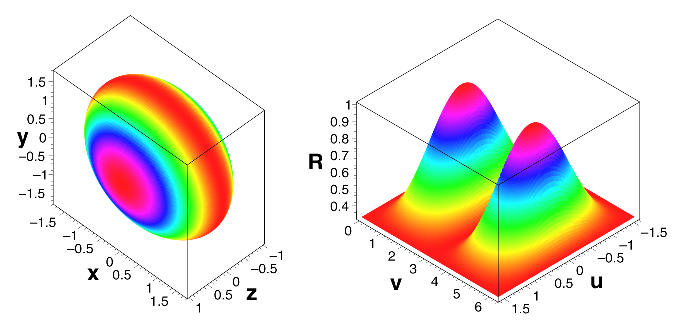
\epsfig{file=chapters/Curvature/ellipsoid_Req, height=50mm}
\end{center}
\vspace{-10pt}
\caption{Similarity curvature for a parameterized ellipsoid with two equal axes.}
\label{fig:curvature-ellipsoid-Req}
\end{figure}
%+++++++++++++++++++++++++++++++++++++++++

Figure~\ref{fig:curvature-ellipsoid-Req} shows results for the same ellipsoid
parameterization when $a=\sqrt{3}$, $b=\sqrt{3}$, and $c=1$. It is interesting to note
that, in comparison with the previous example, since this ellipsoid has two equal length
axes, similarity curvature now takes the sphere curvature value $(1,0)$ only at exactly two
points.\\

